%Dave's handout 3.2 Chain Rule (page 2; Ex from Pg 208#56 from the textbook)
\vspace{-0.25 in}
\begin{framed}
\subsection*{Objectives}
\begin{itemize}
    \item Understand the method of \emph{implicit differentiation} and when it is appropriate to use it to determine $\displaystyle\frac{dy}{dx}$.
    \item Use \emph{implicit differentiation} to determine the equation of a tangent line.
    %\item Be able to apply the concept and method of \emph{implicit differentiation} to real-word problems.
\end{itemize}

%%%Reading Assignment%%%
\subsection*{Suggested Reading:}
\begin{itemize}
\item \cite{Calaway}\footnotemark[1]
   \begin{itemize}
        \item \emph{Section 2.11 Implicit Differentiation and Related Rates}
        \begin{itemize}
            \item Skip \emph{Related Rates} which is the topic covered in lesson \ref{productQuotient}.
        \end{itemize}
    \end{itemize}

\item \cite{openstax}\footnotemark[2]\textsuperscript{,}\footnotemark[3]
    \begin{itemize}
        \item \emph{Section 3.8 Implicit Differentiation}
    \end{itemize}
\end{itemize}
%\subsection*{Supplemental Materials:}
%%%Key Terms%%%
\subsection*{Key Terms and Concepts:} 

\begin{multicols}{2}
\begin{itemize}
    \item Explicit vs. implicit relationships
    \item Implicit differentiation technique
\end{itemize}
\end{multicols}
\end{framed}
\footnotetext[1]{Available free to download from \url{http://www.opentextbookstore.com/details.php?id=14} .}
\footnotetext[2]{Available free to download from \url{https://openstax.org/details/books/calculus-volume-1} .}
\footnotetext[3]{Disregard any examples with trigonometry.}

\newpage
%%%%%%%%%%START LESSON CONTENT%%%%%%%%%%%%%
%\noindent\makebox[\linewidth]{\rule{\textwidth}{0.8pt}}
\Opensolutionfile{ans}[ans12]
\Opensolutionfile{ansL}[ansL12]
%%%%%%%%%%%%%%%%Start First Topic%%%%%%%%%%%%%%%%%%%%%%%%%%%%%
\noindent The Chain Rule was introduced in lesson \ref{GenPower} using the prime notation. You have learned how to use the Chain Rule with the Power Rule. The combination of the two rules is so called the General Power Rule. The \emph{Leibniz} notation was also introduced to help with the intuition of the Chain Rule. In this lesson, we will learn how to use the \textbf{Chain Rule} in a more complex way----with the \textbf{Product Rule} and with the \textbf{Quotient Rule}.\\
\newline
%%%%%%%%%%%%%%%%Start First Topic%%%%%%%%%%%%%%%%%%%%%%%%%%%%%
%%%%%%%%%%%%%%%Dave's handout 3.3.%%%%%%%%%%%%%%%%%%%%%%%%%
\noindent To this point, we have dealt with functions in which the value of y is described \textbf{"explicitly"} as a function $x: y=f(x)$.  We say that x and y have a functional relationship.  In some applications, the relationship between x and y is described by an equation (ex. $x^2+y^2=5$).  In this case, we say that $y$ is defined \textbf{“implicitly”} in terms of $x$, since an assignment of a specific value for $x$ will determine a value or values for $y$. Our interest will still be in determining slopes of tangent lines to curves and in the rate of change of $y$ with respect to $x$, that is, the derivative $\displaystyle\frac{dy}{dx}$.  However, the technique for determining $\displaystyle\frac{dy}{dx}$ will need to be modified from the previous approach when the relationship was explicitly stated. \\
\newline
%%%%%%%%%%%%%%%OpenStax Calculus Vol.1; 3.8 Implicit Differentiation; page 311
\begin{tcolorbox}[title = {Problem-Solving Strategy: Implicit Differentiation}]

\noindent To perform implicit differentiation on an equation that defines a function $y$ implicitly in terms of a variable $x$, use the following steps:
\begin{enumerate}[leftmargin=*]
    \item Take the derivative of both sides of the equation. Keep in mind that $\bm{y}$ \textbf{is a function of} $\bm{x}$ even if we cannot \emph{explicitly} solve for $y$.
    \item Rewrite the equation so that all terms containing $\displaystyle\frac{dy}{dx}$ are on the left and all terms that do not contain $\displaystyle\frac{dy}{dx}$ are on the right.
    \item Factor out $\displaystyle\frac{dy}{dx}$ on the left.
    \item Solve for $\displaystyle\frac{dy}{dx}$ by dividing both sides of the equation by an appropriate algebraic expression.
\end{enumerate}

\end{tcolorbox}
\vspace{0.75cm}
\newpage
%%%%%%%%%Example 2 from Calaway; Applied Calculus; 2.11 Implicit Differentiation and Related Rates%%%%%%%%%%
\begin{comment}
\begin{wrapfigure}[2]{r}{0.5\textwidth}
\includegraphics[width=0.7\textwidth]{images/implicitDiff/implicitCircle.png}
\end{wrapfigure}
\hfill \break
%\vspace{-0.75in}
\end{comment}
\begin{example}
Find the slope of the tangent line to the graph of the equation $x^2+y^2=25$ at the point $(3,4)$.   Then, find the equation of the tangent line at the point.
    %%short answer
    \begin{sol}
    $\displaystyle\frac{dy}{dx}=-\displaystyle\frac{x}{y}$; slope$=-\displaystyle\frac{3}{4}$; $y=-\dfrac{3}{4}x+\dfrac{25}{4}$
    \end{sol}
    %%solution
    \begin{solL}
    Complete solution here.....
    
    \end{solL}
    
\end{example}
\begin{figure}[h!]
 \flushleft
    \includegraphics[scale=0.35]{images//implicitDiff/implicitCircle.png}
    \end{figure}
%%%%%%%%%%%%%%%%%%%%%%%%%%%%%%%%%%%%%%%
\newpage
 \begin{figure}[h!]
 \centering
    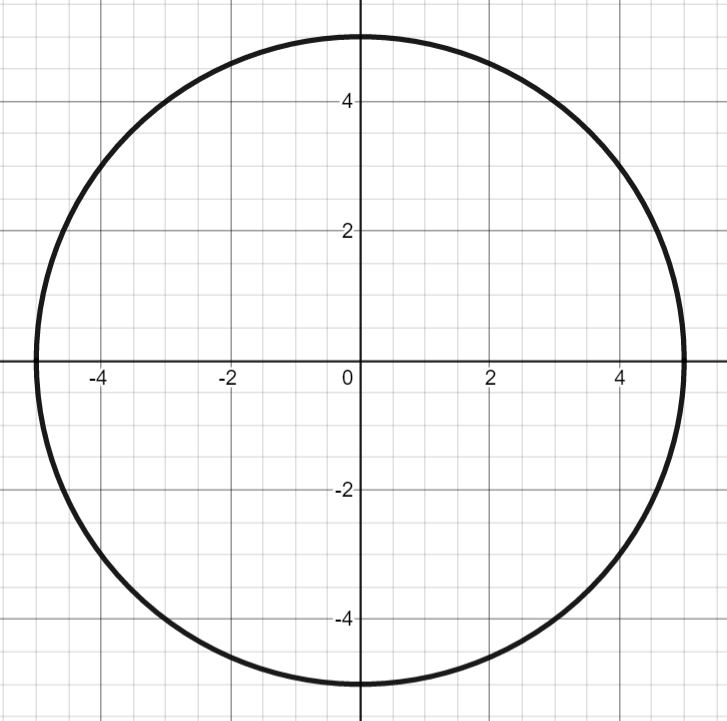
\includegraphics[scale=0.45]{images/implicitDiff/implicit12_1a.PNG}
    \caption{Example 12.1a}
    \end{figure}
 \vspace{1cm}   
    \begin{figure}[h!]
 \centering
    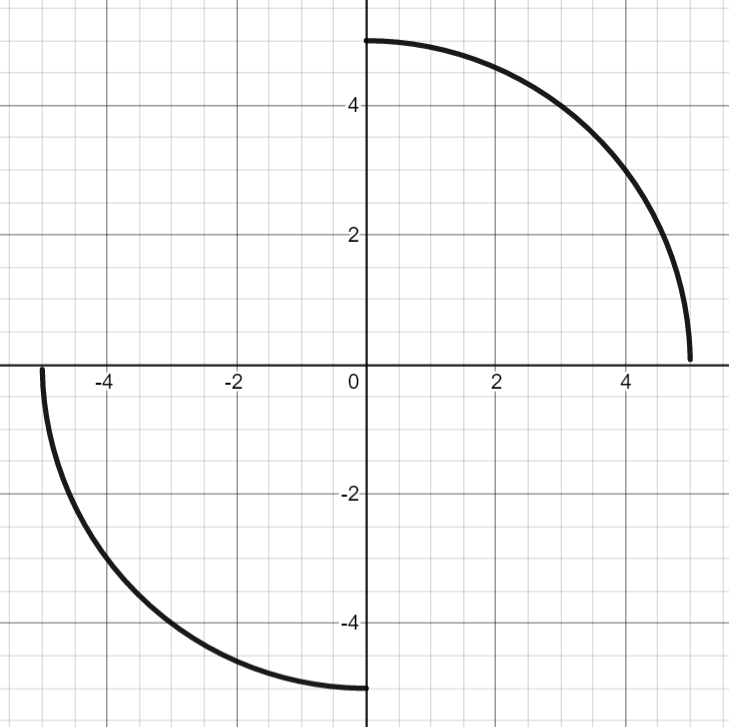
\includegraphics[scale=0.45]{images/implicitDiff/implicit12_1b.PNG}
    \caption{Example 12.1b}
    \end{figure}
\vspace{1cm}
      \begin{figure}[h!]
 \centering
    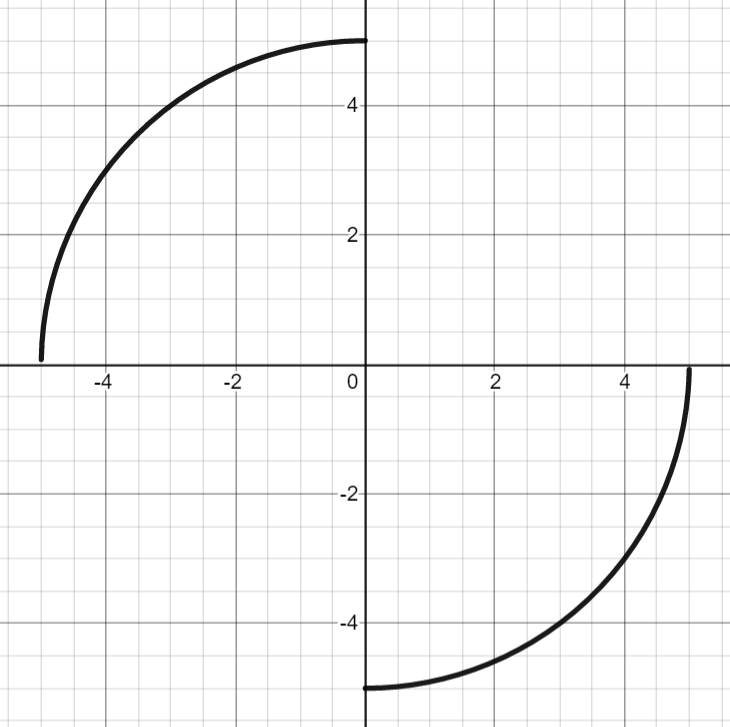
\includegraphics[scale=0.45]{images/implicitDiff/implicit12_1c.PNG}
    \caption{Example 12.1c}
    \end{figure}
\newpage
%%%%%%%%%%%%%%%%%%%%%%%%
\begin{example}
 If $x$ and $y$ are related by the equation $xy^2=10$, answer the following questions:
\renewcommand{\labelenumi}{\textbf{(\alph{enumi})}}
\begin{enumerate}[leftmargin=*]
    \item Find $\displaystyle\frac{dy}{dx}$.
    \item Evaluate: $\left.\displaystyle\frac{dy}{dx}\right\rvert_{(2,-\sqrt{5})}$ and interpret the result.
\end{enumerate}
    %%short answer
    \begin{sol}
    \onehalfspacing{
    \begin{enumInline1}
    \item $\displaystyle\frac{dy}{dx}=-\displaystyle\frac{y}{2x}$ 
    \item $\displaystyle\frac{\sqrt{5}}{4}$; slope of the tangent line at this point.
    \end{enumInline1} }
    \end{sol}
    %%solution
    \begin{solL}
    Complete solution here.....
    
    \end{solL}
    
\end{example}
\vspace*{\stretch{2}}
\newpage
 \begin{figure}[h!]
 \centering
    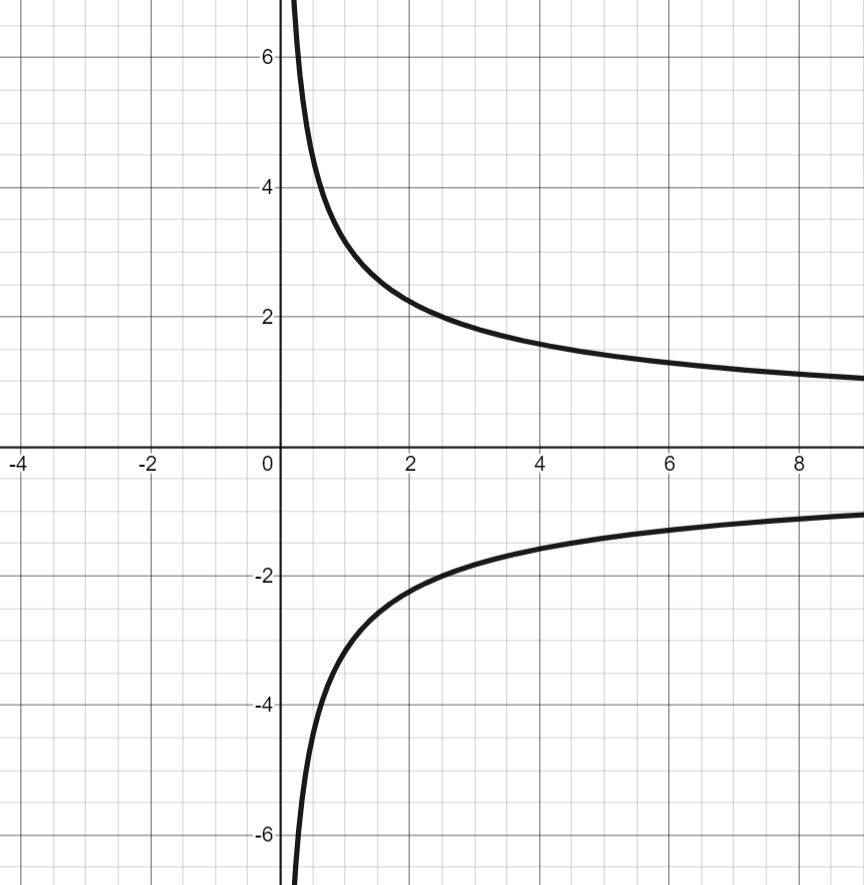
\includegraphics[scale=0.45]{images/implicitDiff/implicit12_2a.PNG}
    \caption{Example 12.2a}
    \end{figure}
    
    \begin{figure}[h!]
 \centering
    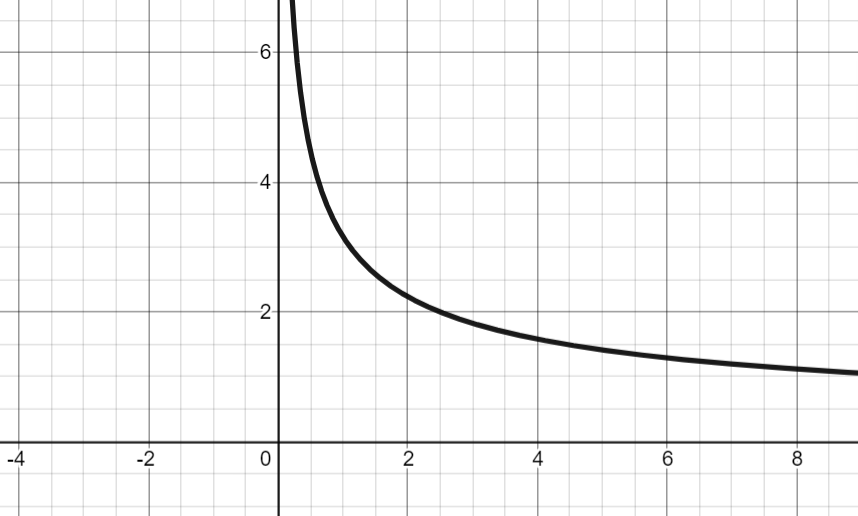
\includegraphics[scale=0.45]{images/implicitDiff/implicit12_2b.PNG}
    \caption{Example 12.2b}
    \end{figure}
      \begin{figure}[h!]
 \centering
    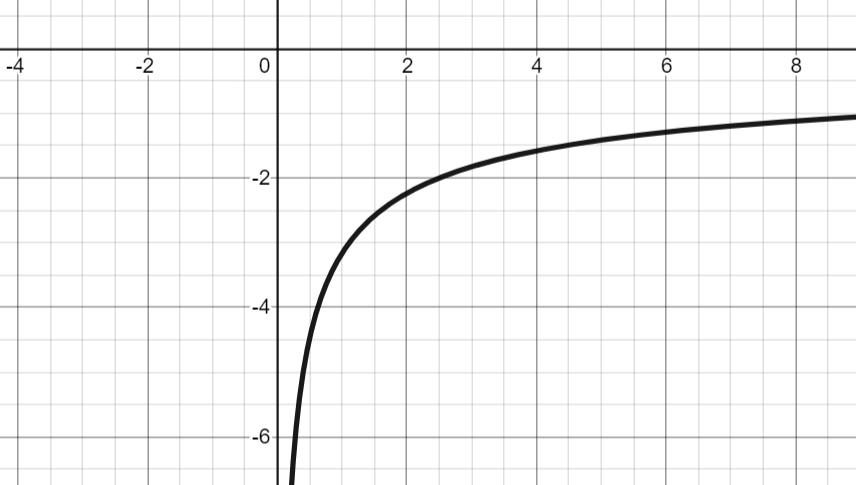
\includegraphics[scale=0.45]{images/implicitDiff/implicit12_2c.PNG}
    \caption{Example 12.2c}
    \end{figure}



%%%%%%%%%%%%End Examples%%%%%%%%%%%%%%%%%%
%%%%%%%%%%%%%%%End Topic%%%%%%%%%%%%%%%%%%



%%%%%%%%%%%%%%%End Lesson%%%%%%%%%%%%%%%%%%
\Closesolutionfile{ans}
\Closesolutionfile{ansL}

%%%Short Answers to Examples%%%
\vspace*{\fill}

\subsection*{Short Answers to Examples}
%\vspace{-0.25cm}
%\begin{multicols}{2}
\input{ans12}
%\end{multicols}


